\vspace{10pt}
\section{Design Methodology}\label{sec:framwork}
Based on the analysis of Section~\ref{sec:w_and_r}, a new design flow are proposed to explore the design space of the cross-point ReRAM array, which  is shown in Figure~\ref{fig:FlowChart}. Generally, the flow can be summarized as two stages: initialization stage and the computation stage. At the initialization stage, the physical parameters, including the resistances of the ReRAM cell, interconnect wires and pull up resistors, the threshold voltage of the ReRAM cell, as well as non-linearity coefficients, are firstly input. All of this parameters are determined by materials and the process technology. Thus they and can not be changed easily during the design of memory array. After that, the design constraints should be decided according to the area/energy budgets and different applications. Then, based on these data, the original version of coefficients matrix $A_{basic}$ and the vector of constant terms $C_{basic}$ are set up. Since the value of $A_{basic}$ and $C_{basic}$ do not consider the edge conditions of the write/read schemes and therefore do not change during the design space exploration, their value are saved at this step. Then the programming schemes are chosen. The designer can either explores all of the possible programming schemes or chooses proper schemes according to the prior experience observed in our study (For example, we have already shown that the one bit write operation is more suitable for an area-constrainted design than multi bit write). Then the final step of the initialization stage is to adjust the coefficients in $A_{basic}$ and $C_{basic}$ base on edge conditions. 



\begin{figure}[!t]
\centering
  % Requires \usepackage{graphicx}
  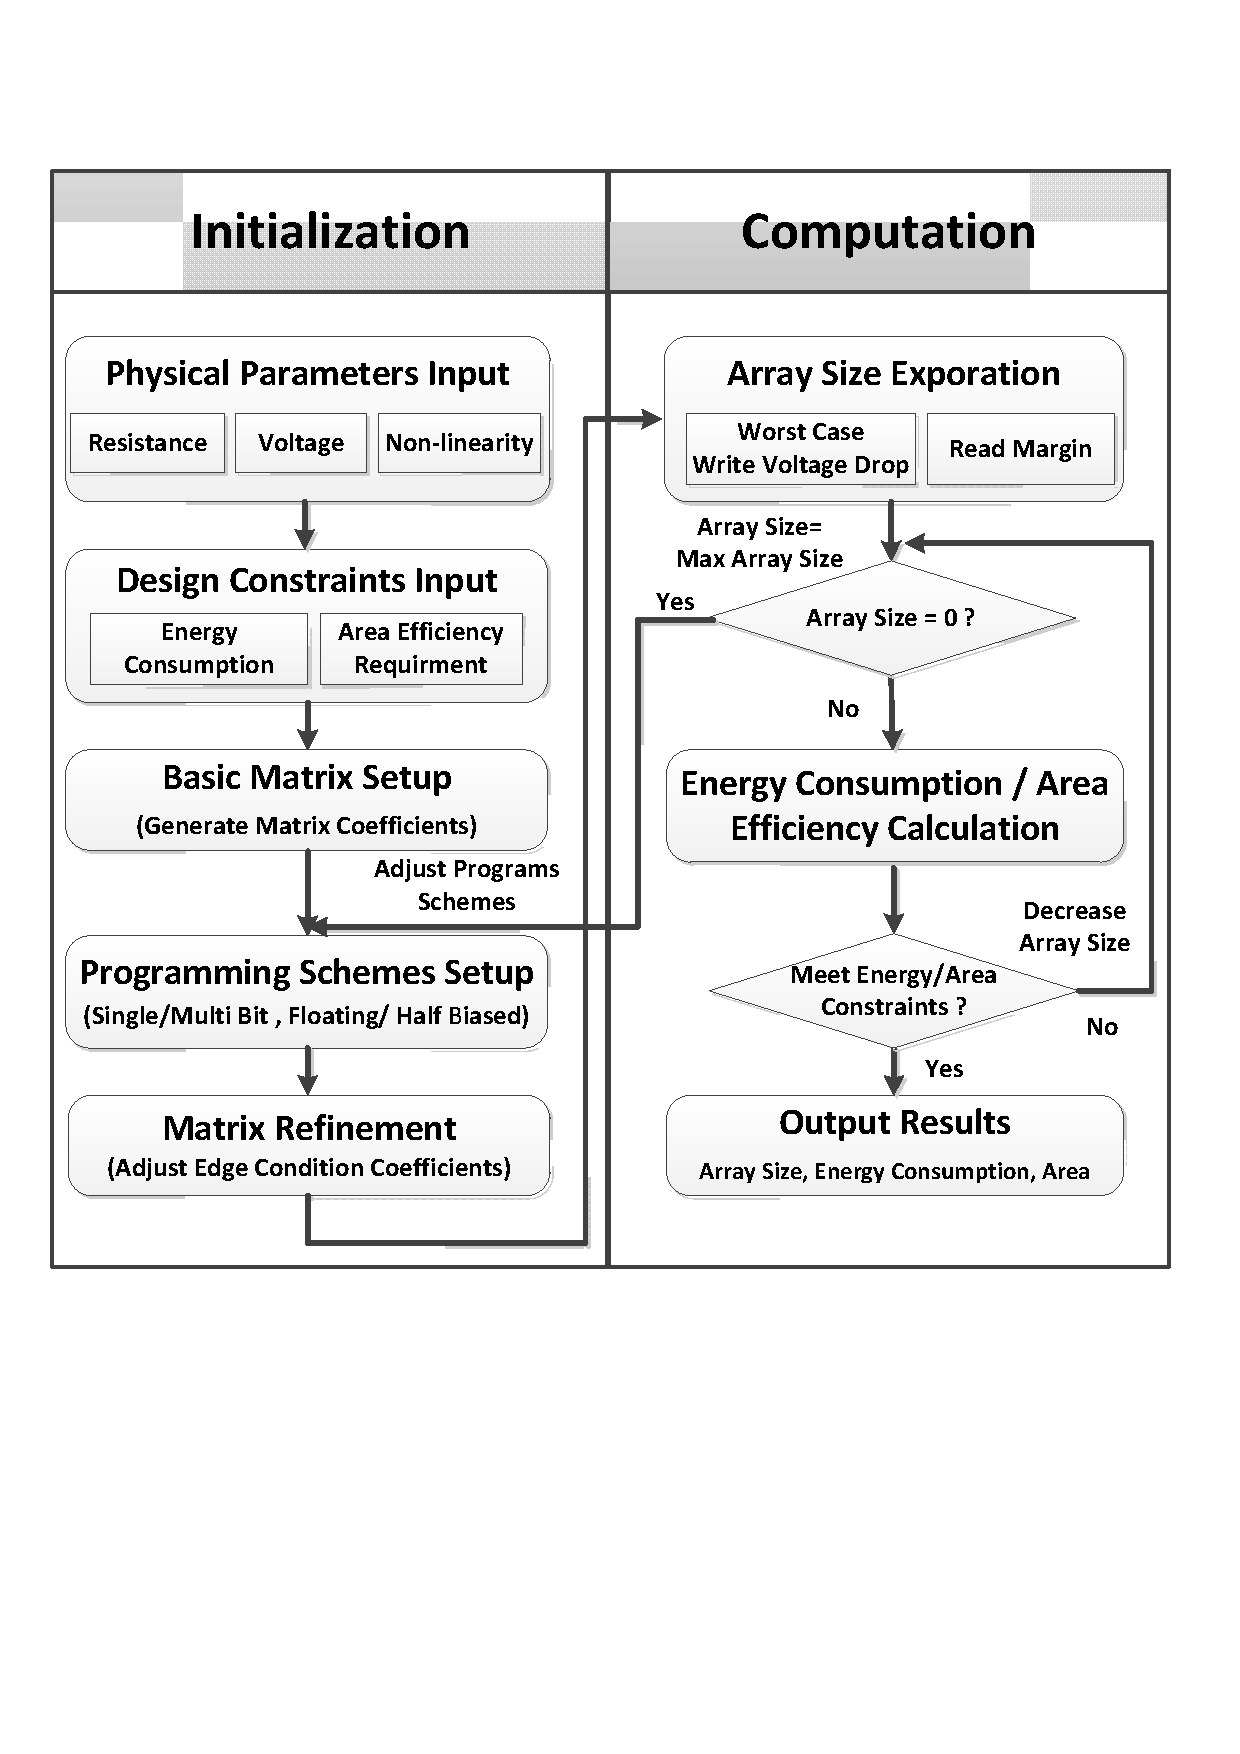
\includegraphics[width=0.5\textwidth]{./figures/FlowChart.pdf}\\
  \caption{The Proposed Design Flow of Design Space Exploration for ReRAM based Cross-point Array.}\label{fig:FlowChart}
\end{figure}
